%% Submissions for peer-review must enable line-numbering
%% using the lineno option in the \documentclass command.
%%
%% Preprints and camera-ready submissions do not need
%% line numbers, and should have this option removed.
%%
%% Please note that the line numbering option requires
%% version 1.1 or newer of the wlpeerj.cls file.

\documentclass[fleqn,10pt,lineno]{wlpeerj} % for journal submissions
% \documentclass[fleqn,10pt]{wlpeerj} % for preprint submissions

\newcommand{\cheng}[1]{\textcolor{green}{\textbf{Cheng: }{\footnotesize #1}}}
\newcommand{\alasdair}[1]{\textcolor{blue}{\textbf{Alasdair: }{\footnotesize #1}}}

\usepackage{bm} % bold math symbols
\usepackage{hyperref} % create hyperlinks
\usepackage[labelfont=bf]{caption} % figure captions
\usepackage{algorithm} 
\usepackage{algpseudocode} % display algorithms in pseudo-code

\hypersetup{
	colorlinks   = true, % Colours links instead of ugly boxes
	pdfauthor    = {Alasdair Tran and Cheng Soon Ong},
	pdftitle	 = {Combining Active Learning Suggestions},
}

\DeclareMathAlphabet{\mathcal}{OMS}{cmsy}{m}{n} % reset caligraphy font

% some convenient symbols
\DeclareMathOperator{\Beta}{Beta}
\DeclareMathOperator{\Bin}{Bin}
\DeclareMathOperator{\tr}{tr}
\newcommand{\A}{\mathpzc{A}}
\newcommand{\B}{\mathcal{B}}
\newcommand{\X}{\mathcal{X}}
\newcommand{\Y}{\mathcal{Y}}
\newcommand{\Ecal}{\mathcal{E}}
\newcommand{\Normal}{\mathcal{N}}
\newcommand{\Unlabelled}{\mathcal{U}}
\newcommand{\Labelled}{\mathcal{L}}
\newcommand{\R}{\mathcal{R}}
\newcommand*{\argmin}{\operatornamewithlimits{argmin}\limits}
\newcommand*{\argmax}{\operatornamewithlimits{argmax}\limits}


\title{Combining Active Learning Suggestions}

\author[1]{Alasdair Tran}
\author[2]{Cheng Soon Ong}
\affil[1]{}
\affil[2]{Machine Learning Research Group, Data61, CSIRO, Australia}

\keywords{machine learning, astronomy, active learning, bandit, rank aggregation}

\begin{abstract}
Recent advances in sensors and scientific instruments have led to an increasing
use of machine learning techniques for managing the data deluge. Supervised
learning has become a widely used paradigm in many big data applications.
However,  labeled examples are required during the training phase of supervised
machine learning algorithms, and the labeling has become a  significant
bottleneck. This paper explores the use of machine learning algorithms for
identifying informative examples for labeling, the so-called active learning
setting. We  empirically compare several active learning heuristics on
benchmark UCI datasets, and focus on its  application to photometric classification
of the Sloan Digital Sky Survey. By considering each  active learning heuristic
as an expert recommendation of which example to label, we propose to  combine
them using bandit and rank aggregation algorithms. Our results show that
combining  active learning suggestions improves over each individual heuristic
(including passive  learning), and provides a promising practical approach.

\end{abstract}

\begin{document}

\flushbottom
\maketitle
\thispagestyle{empty}

\section*{Introduction}

There are three ideas which are often used to elicit human responses - active
learning, bandits, and experimental designs. Although similar in spirit, these
ideas have different foundations which lead to different formulations. Related
to this but with literature from a different field is social choice theory,
which looks at how individual preferences are aggregated.

Active learning considers the setting where the agent interacts with its
environment to procure a training set. This contrasts with passive learning,
where the agent passively receives i.i.d. samples from some underlying
distribution. The environment is usually assumed to be infinite and the agent
has to choose a location to query an oracle for a label. It is often assumed
that there is no noise in the label, and hence there is no benefit of querying
the same point again. In many practical applications, the environment is
considered to be finite (but large). This is called the pool-based active
learning.

A bandit problem is a sequential allocation problem defined by a set of
actions. The agent chooses an action at each time step, and the environment
returns a reward. The aim of the agent is to maximise reward. In basic
settings, the set of actions is considered to be finite. There are three
fundamental formalisations of the bandit problem, depending on the assumed
nature of the reward process: stochastic, adversarial and Markovian. In all
three settings the reward is uncertain, and hence the agent may have to play a
particular action repeatedly. The agent is compared to a static agent which has
played the best action. This difference in reward is called regret.

In contrast to active learning, experimental design considers the problem of
regression, i.e. where the label $y\in R$ is a real number. The problem to be
solved in experimental design is to choose a set of trials (say of size N) to
gather enough information about the object of interest. The goal is to maximise
the information obtained about the parameters of the model (of the object). It
is often assumed that the observations at the N trials are independent. When N
is finite this is called exact design, otherwise it is called approximate or
continuous design. The environment is assumed to be infinite (e.g. $R^d$) and
the observations are scalar real variables.

Previous surveys~\cite{baram04, hsu15}.
We are more comprehensive, and consider other types of combination.

\section*{Problem Formulation}

\subsection*{Active Learning Suggestions}

Suppose we have a hypothesis $h$ that maps the input space $\X \subset \mathbb{R}^d$
to the label space $\Y$. We require that a small number of objects have already
been labelled--these become the labelled set $\Labelled \subset \X \times \Y$.
The rest form the unabelled set
$\Unlabelled \subset \X$. Now consider the problem of choosing the next example
in $\Unlabelled$ for querying, using a rule
$r(\bm{x}; h)$ that gives each unlabelled example a score based only on
their feature vector $\bm{x}$ and the current hypothesis $h$. Coming up with a good
rule is itself a hard problem, but there have been many attempts to derive
good heuristics.
Five common ones are listed in Table \ref{tab:heuristics}.
They roughly fall into two categories: uncertainty sampling and version space
reduction.

\cite{lewis94} introduce the idea of uncertainty sampling, where we select the example whose class
membership the classifier is least certain about. These tend to be points that are near the
decision boundary of the classifier. Perhaps the simplest way to quantify uncertainty is \cite{culotta05}'s least confidence heuristic, where we pick the candidate whose most likely label the classifier is most uncertain about. A second option is to calculate the
entropy \citep{shannon48}, which measures the amount of information needed to encode a distribution.
Intuitively, the closer class probabilities of an object are to random guessing, the higher its
entropy will be. This gives us the heuristic of picking the candidate with the highest entropy.
Finally we can pick the candidate with the smallest margin, which is defined to be the difference between the two highest class probabilities \citep{scheffer01} Since the sum of all probabilities must be 1, the smaller the margin is, the more uncertain we are about the object's class membership. 

Instead of focussing on the uncertainty of individual predictions, we could
instead try to constrain the size of the version space, thus allowing the search for the optimal
hypothesis to be more precise. The version space is defined as the set of all possible hypotheses that are consistent with the current training set. To quantify the size the space, we can train a committee of
classifiers, $\B = \{h_1, h_2, ..., h_B\}$, and measure the disagreement among the members about an
object's class membership. Each committee member needs to have a hypothesis that is as different
from the others as possible but that is still in the version space \cite{melville04}. In order to
have this diversity, we give each member only a subset of the training examples. Since there might
not be enough training data, we need to use bootstrapping and select samples with replacement. Hence
this method is often called Query by Bagging (QBB).

One way to measure the level of disagreement is to calculate the margin using the class
probabilities estimated by the committee \cite{melville04}. This looks similar to one of the
uncertainty sampling heuristics, except now we first average out the probabilities of the members
before minimising the margin. \cite{mccallum98} offer an alternative disagreement measure which
involves picking the candidate with the largest expected Kullback--Leibler (KL) divergence from the average.

\begin{table}[h]
	\caption {Summary of active learning heuristics used in our experiments} \label{tab:heuristics}
	\centering
	\begin{tabular}{lll}
		\toprule
		{Heuristic}  &  Objective  \\
		\midrule
        Least Confidence &
			$\argmax_{x \in \Ecal} \left\{ \max_{y \in \Y} p(y | \bm{x}; \B) \right\}$
			\\
		Highest Entropy &
			$\argmax_{x \in \Ecal} \left\{-\sum_{y \in \Y} p(y | \bm{x}; h)
            \log \big[ p(y | \bm{x}; h) \big] \right\}$
			\\[2ex]
		Smallest Margin &
			$\argmin_{x \in \Ecal} \left\{ \max_{y \in \Y} p(y | \bm{x}; h) -
            \max_{z \in \Y \setminus \{y\}} p(z | \bm{x}; h)  \right\}$
			\\[2ex]
		Smallest QBB Margin &
			$\argmin_{x \in \Ecal} \left\{ \max_{y \in \Y} p(y | \bm{x}; \B) -
            \max_{z \in \Y \setminus \{y\}} p(z | \bm{x}; \B)  \right\}$
			\\[2ex]
		Largest QBB KL &
			$\argmax_{x \in \Ecal} \left\{ \dfrac{1}{B}
               \sum_{b=1}^B D_{\mathrm{KL}}(p_b\|p_\B) \right\}$
			\\
		\bottomrule
	\end{tabular}
\end{table}

\subsection*{Combining the Suggestions with Bandits}

Out of the five heuristics discussed, how do we know which one is the optimal, anyway? There have
been some attempts in the literature to do a theoretical analysis of them. However proofs are
scarce, and when there is one available, they normally only work under simplifying assumptions. For
example, \cite{freund97} show that the query by committee algorithm (a slight variant of our
QBB heuristics) guarantees an exponential decrease in the prediction error with the training size,
but only under certain restrictions such as there is no noise. Thus whether any of these heuristics
is guaranteed to beat random sampling is still an open question. We shall not worry too much about
the theoretical analysis in this thesis. Instead we shall focus on an empirical analysis in the
astronomical domain.

To help us automatically choose the optimal heuristic, we now turn our attention to the multi-armed
bandit problem in probability theory. The colourful name originates from the situation where a
gambler stands in front of a slot machine with $s$ levers. When pulled, each lever gives out a random
reward according to some unknown distribution. The goal of the game is to come up with a strategy
that can maximise the gambler's lifetime rewards while minimising the number of pulls.

Suppose we have a set of $s$ heuristics $ \R = \{r_1, ..., r_s \}$. Each heuristic has a different
ability to identify the candidate whose labelling information is most valuable. An appropriate
reward is then the incremental increase in the accuracy rate after the candidate is added to the
training set. We assume that the heuristic rewards are independent of each other. This is
reasonable since the theories with which we use to derive the heuristics are mostly unrelated.

One problem in multi-arm bandits is the trade-off between exploring random heuristics and exploiting the best heuristic so far.
There are many instances in which we find our previously held beliefs to
be completely wrong. Thus by always exploiting, we could miss out on the optimal heuristic. On the
other hand, if we explore too much, it might take a long time to reach the desired accuracy and the
strategy ends up being no different from random sampling.

There are two main methods in the literature that address this exploration vs exploitation problem.
The algorithm with a strong theoretical guarantee is Upper Confidence Bound \cite{auer02}. There is also an older algorithm called Thompson sampling \cite{thompson33} that solves the trade-off from a Bayesian perspective first. In this paper we shall consider four variants: Thompson sampling with normally distributed rewards, Optimally Confident UCB \cite{lattimore15}, KL-UCB \cite{cappe13}, and EXP3++ \cite{seldin14}.


\subsection*{Combining the Suggestions with Social Choice Theory}

http://plato.stanford.edu/entries/social-choice/. Pairwise majority rule. Borda count. Geometric mean \cite{bedo14}

\algblock[Name]{Start}{End}
\algblockdefx[Forall]{Foreach}{Endforeach}%
			[1]{\textbf{for each} #1 \textbf{do}}%
			{\textbf{end for}}

\begin{algorithm}[tbp]
	\caption{Thompson sampling} \index{bandit}
	\label{alg:bandit}
	\begin{algorithmic}[1]
		\Procedure {ThompsonSampling}{$\Unlabelled$, $\Labelled_T$, $h$, $n$, $E$,
			                      $\R$, $\bm{\mu}$, $\bm{\sigma}^2$, $\bm{\tau}^2$}
    		\While {$|\Labelled_T| < n$}
        		\Foreach  {$i \in \{1, 2, ..., |\R|\}$}
        			\State $\nu_i' \leftarrow$ draw a sample from $\Normal(\mu_i, \sigma^2_i)$
        		\Endforeach
        		\State $r_* \leftarrow \argmax_{i} \nu_i'$
        		\State $\Ecal$ $\leftarrow$ random sample of size $E$ from $\Unlabelled$
        		\State $\bm{x}_* \leftarrow \argmax_{\bm{x} \in \Ecal} r_*(\bm{x})$
        		\State $y_* \leftarrow$ ask the expert to label $\bm{x}_*$
        		\State $\Labelled_T \leftarrow \Labelled_T  \cup (\bm{x}_*, y_*)$
        		\State $\Unlabelled \leftarrow \Unlabelled \setminus \bm{x}_*$
        		\State $h(\bm{x}) \leftarrow$ retrain the classifier
        		\State $\delta$ $\leftarrow$ incremental increase in the accuracy
        		\State $\mu_* \leftarrow \dfrac{\mu_* \tau^2_* + \delta \sigma^2_*}{\sigma^2_* + \tau^2_*}$
                \State $\sigma_*^2 \leftarrow \dfrac{\sigma^2_* \tau^2_*}{\sigma^2_* + \tau^2_*}$
    		\EndWhile
		\EndProcedure
	\end{algorithmic}
\end{algorithm}





\section*{Empirical comparison}

\subsection*{Description of datasets}

\begin{table}[h]
	\caption {Overview of datasets} \label{tab:datasets}
	\centering
	\begin{tabular}{lrrr}
		\toprule
		{Dataset}  & Size &  Classes & Majority  \\
		\midrule
        \href{https://archive.ics.uci.edu/ml/datasets/Glass+Identification}{glass}
        	& $214$ & $6$ & $33\%$ \\
		\href{https://archive.ics.uci.edu/ml/datasets/Ionosphere}{ionosphere}
        	& $351$ & $2$ & $64\%$ \\
        \href{https://archive.ics.uci.edu/ml/datasets/Breast+Cancer+Wisconsin+(Prognostic)}{iris}
        	& $150$ & $3$ & $33\%$ \\
        \href{https://archive.ics.uci.edu/ml/datasets/MAGIC+Gamma+Telescope}{magic}
        	& $19~020$ & $2$ & $65\%$ \\
        \href{https://archive.ics.uci.edu/ml/datasets/MiniBooNE+particle+identification}{miniboone}
        	& $129~596$ & $2$ & $72\%$ \\
        \href{https://archive.ics.uci.edu/ml/datasets/Page+Blocks+Classification}{pageblock}
        	& $5~473$ & $5$ & $90\%$ \\
		\href{https://archive.ics.uci.edu/ml/datasets/Pima+Indians+Diabetes}{pima}
        	& $733$ & $2$ & $66\%$ \\
        \href{http://dx.doi.org/10.5281/zenodo.58500}{sdss}
        	& $2~801~002$ & $3$ & $61\%$ \\
		\href{https://archive.ics.uci.edu/ml/datasets/Connectionist+Bench+(Sonar,+Mines+vs.+Rocks)}{sonar}
        	& $208$ & $2$ & $53\%$ \\
        \href{https://archive.ics.uci.edu/ml/datasets/Statlog+(Vehicle+Silhouettes)}{vehicle}
        	& $846$ & $4$ & $26\%$ \\
        \href{https://archive.ics.uci.edu/ml/datasets/Wine}{wine}
        	& $178$ & $3$ & $40\%$ \\
		\href{https://archive.ics.uci.edu/ml/datasets/Breast+Cancer+Wisconsin+(Prognostic)}{wpbc}
        	& $194$ & $2$ & $76\%$ \\
		\bottomrule
	\end{tabular}
\end{table}

\subsubsection*{Experimental Setup}

Reward: improvement in balanced accuracy. Posterior balanced Accuracy derivation.

\begin{figure}[tbp]
	\centering
	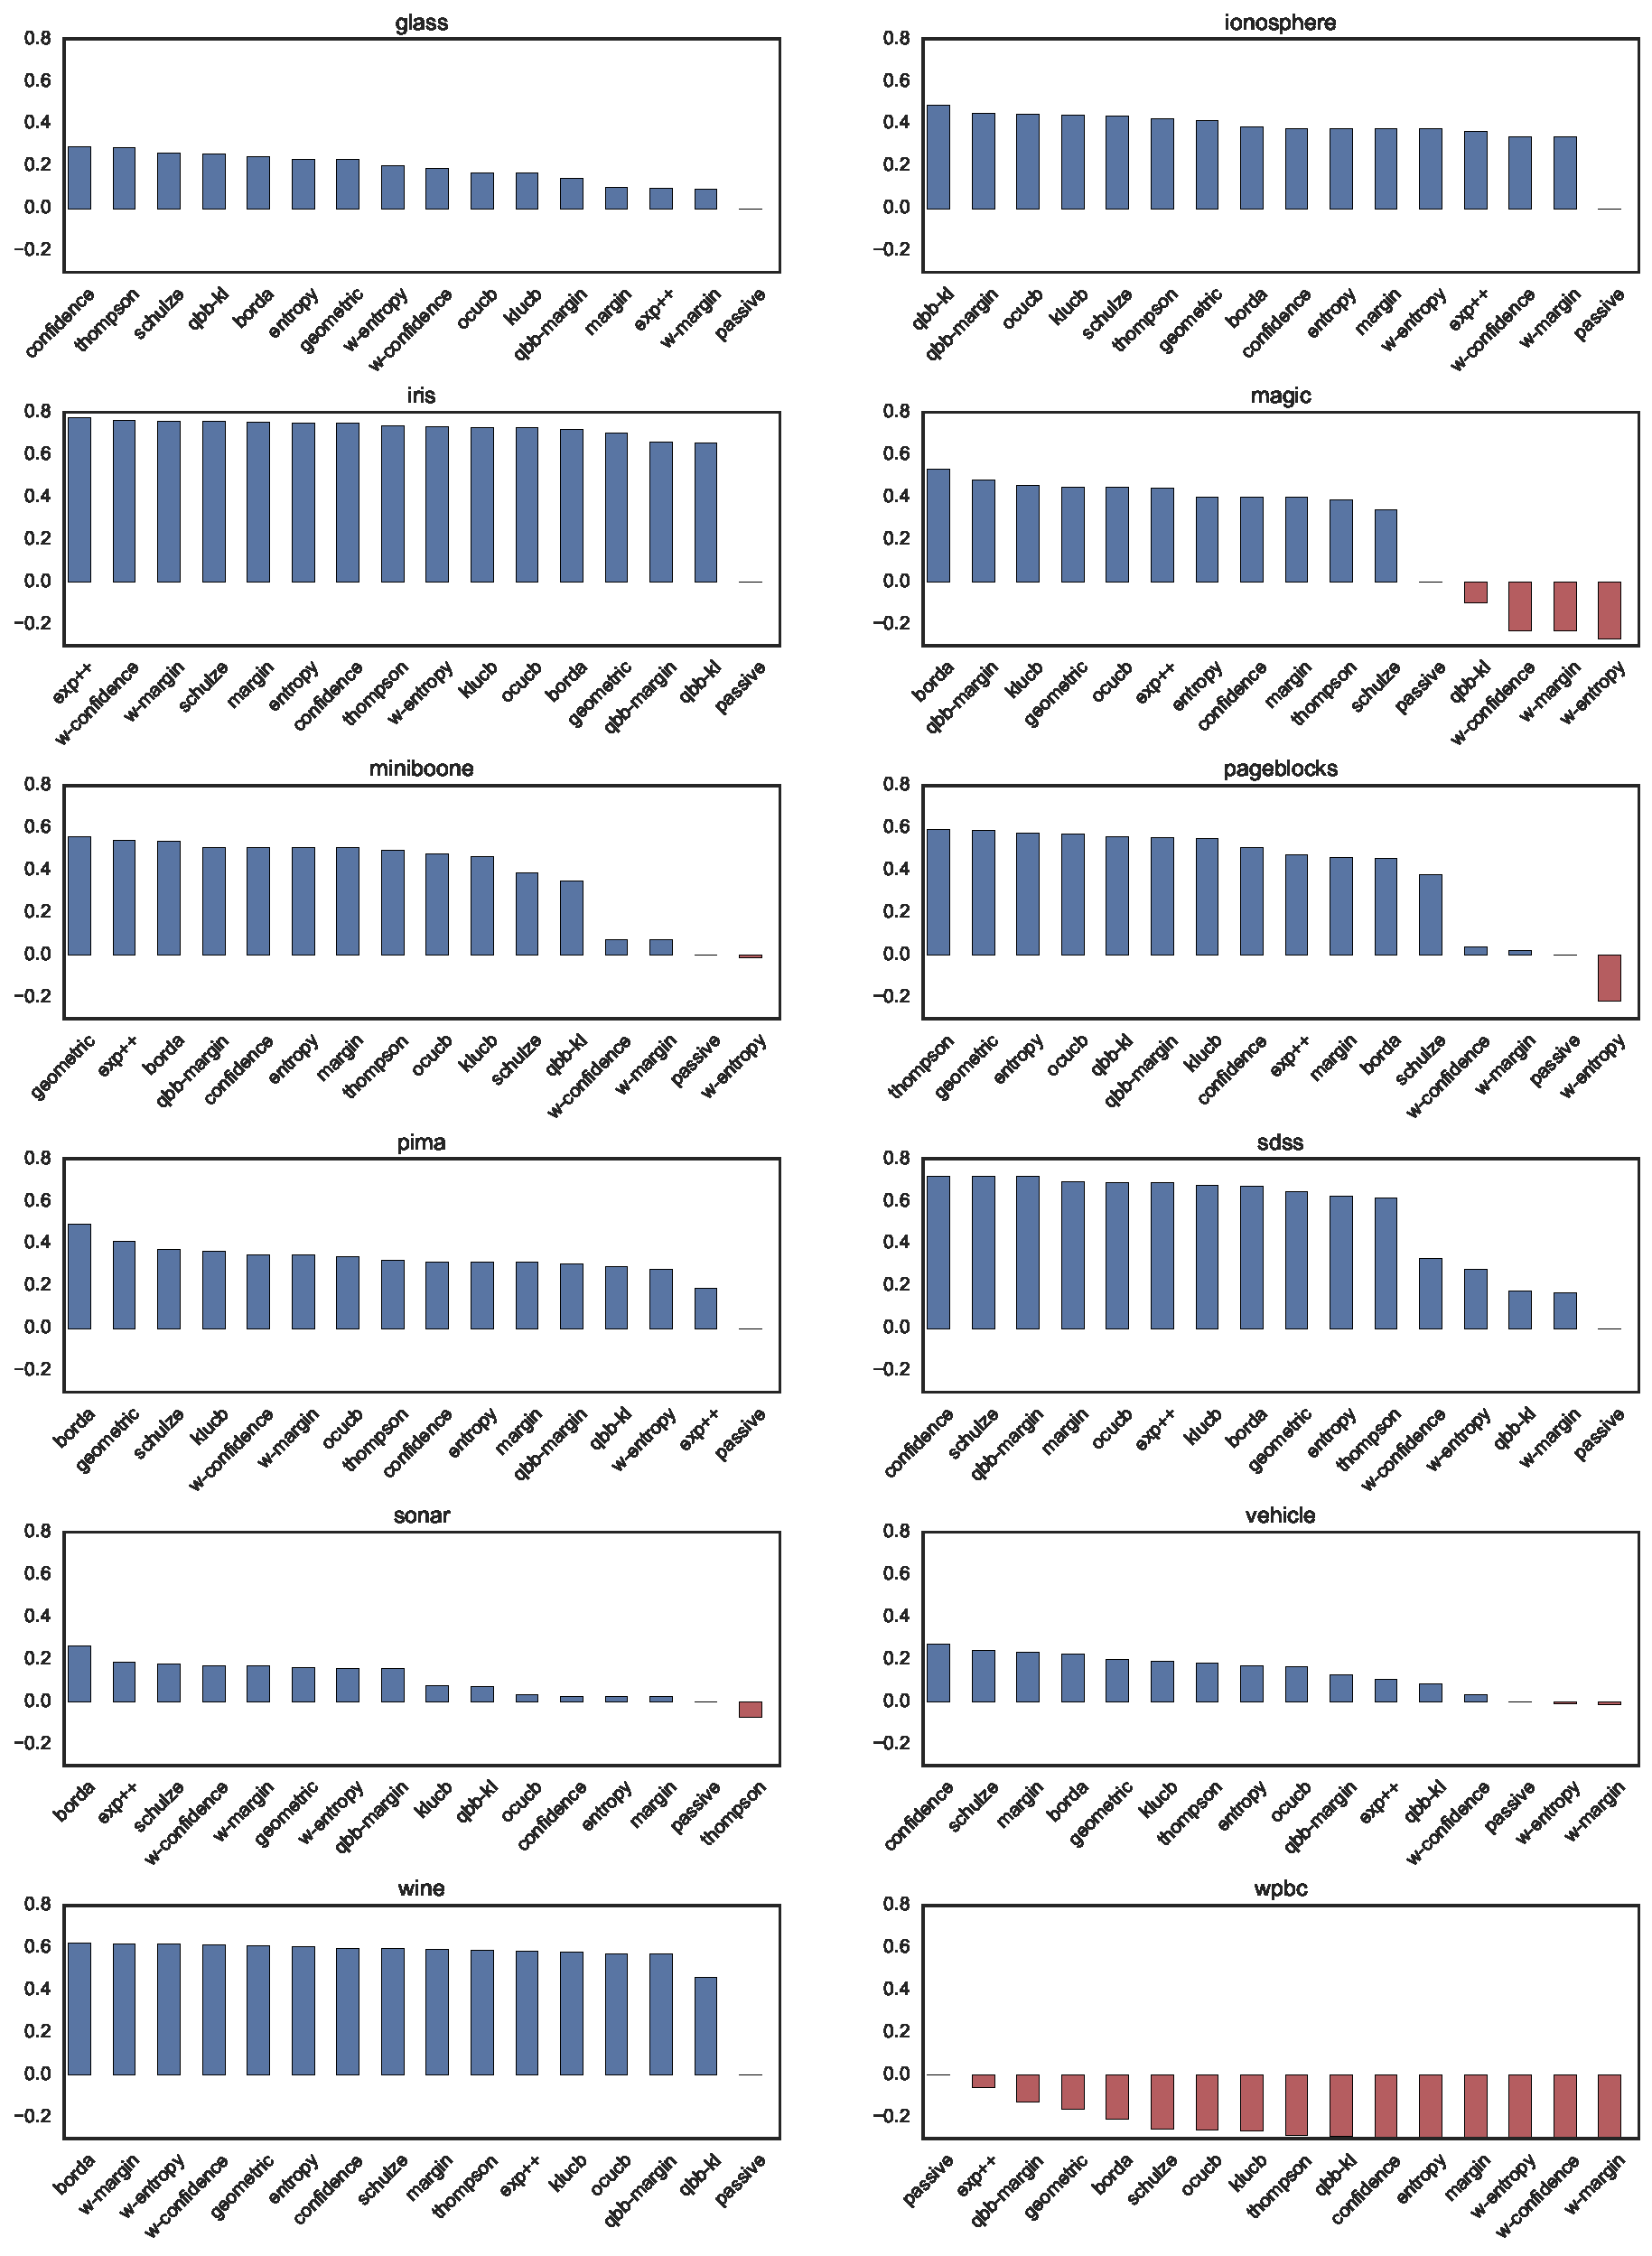
\includegraphics[width=\textwidth]{figures/strengths}
	\caption[Policy strength]{Strength of policies and heuristics relative to passive learning}
	\label{fig:strengths}
\end{figure}


\begin{figure}[tbp]
	\centering
	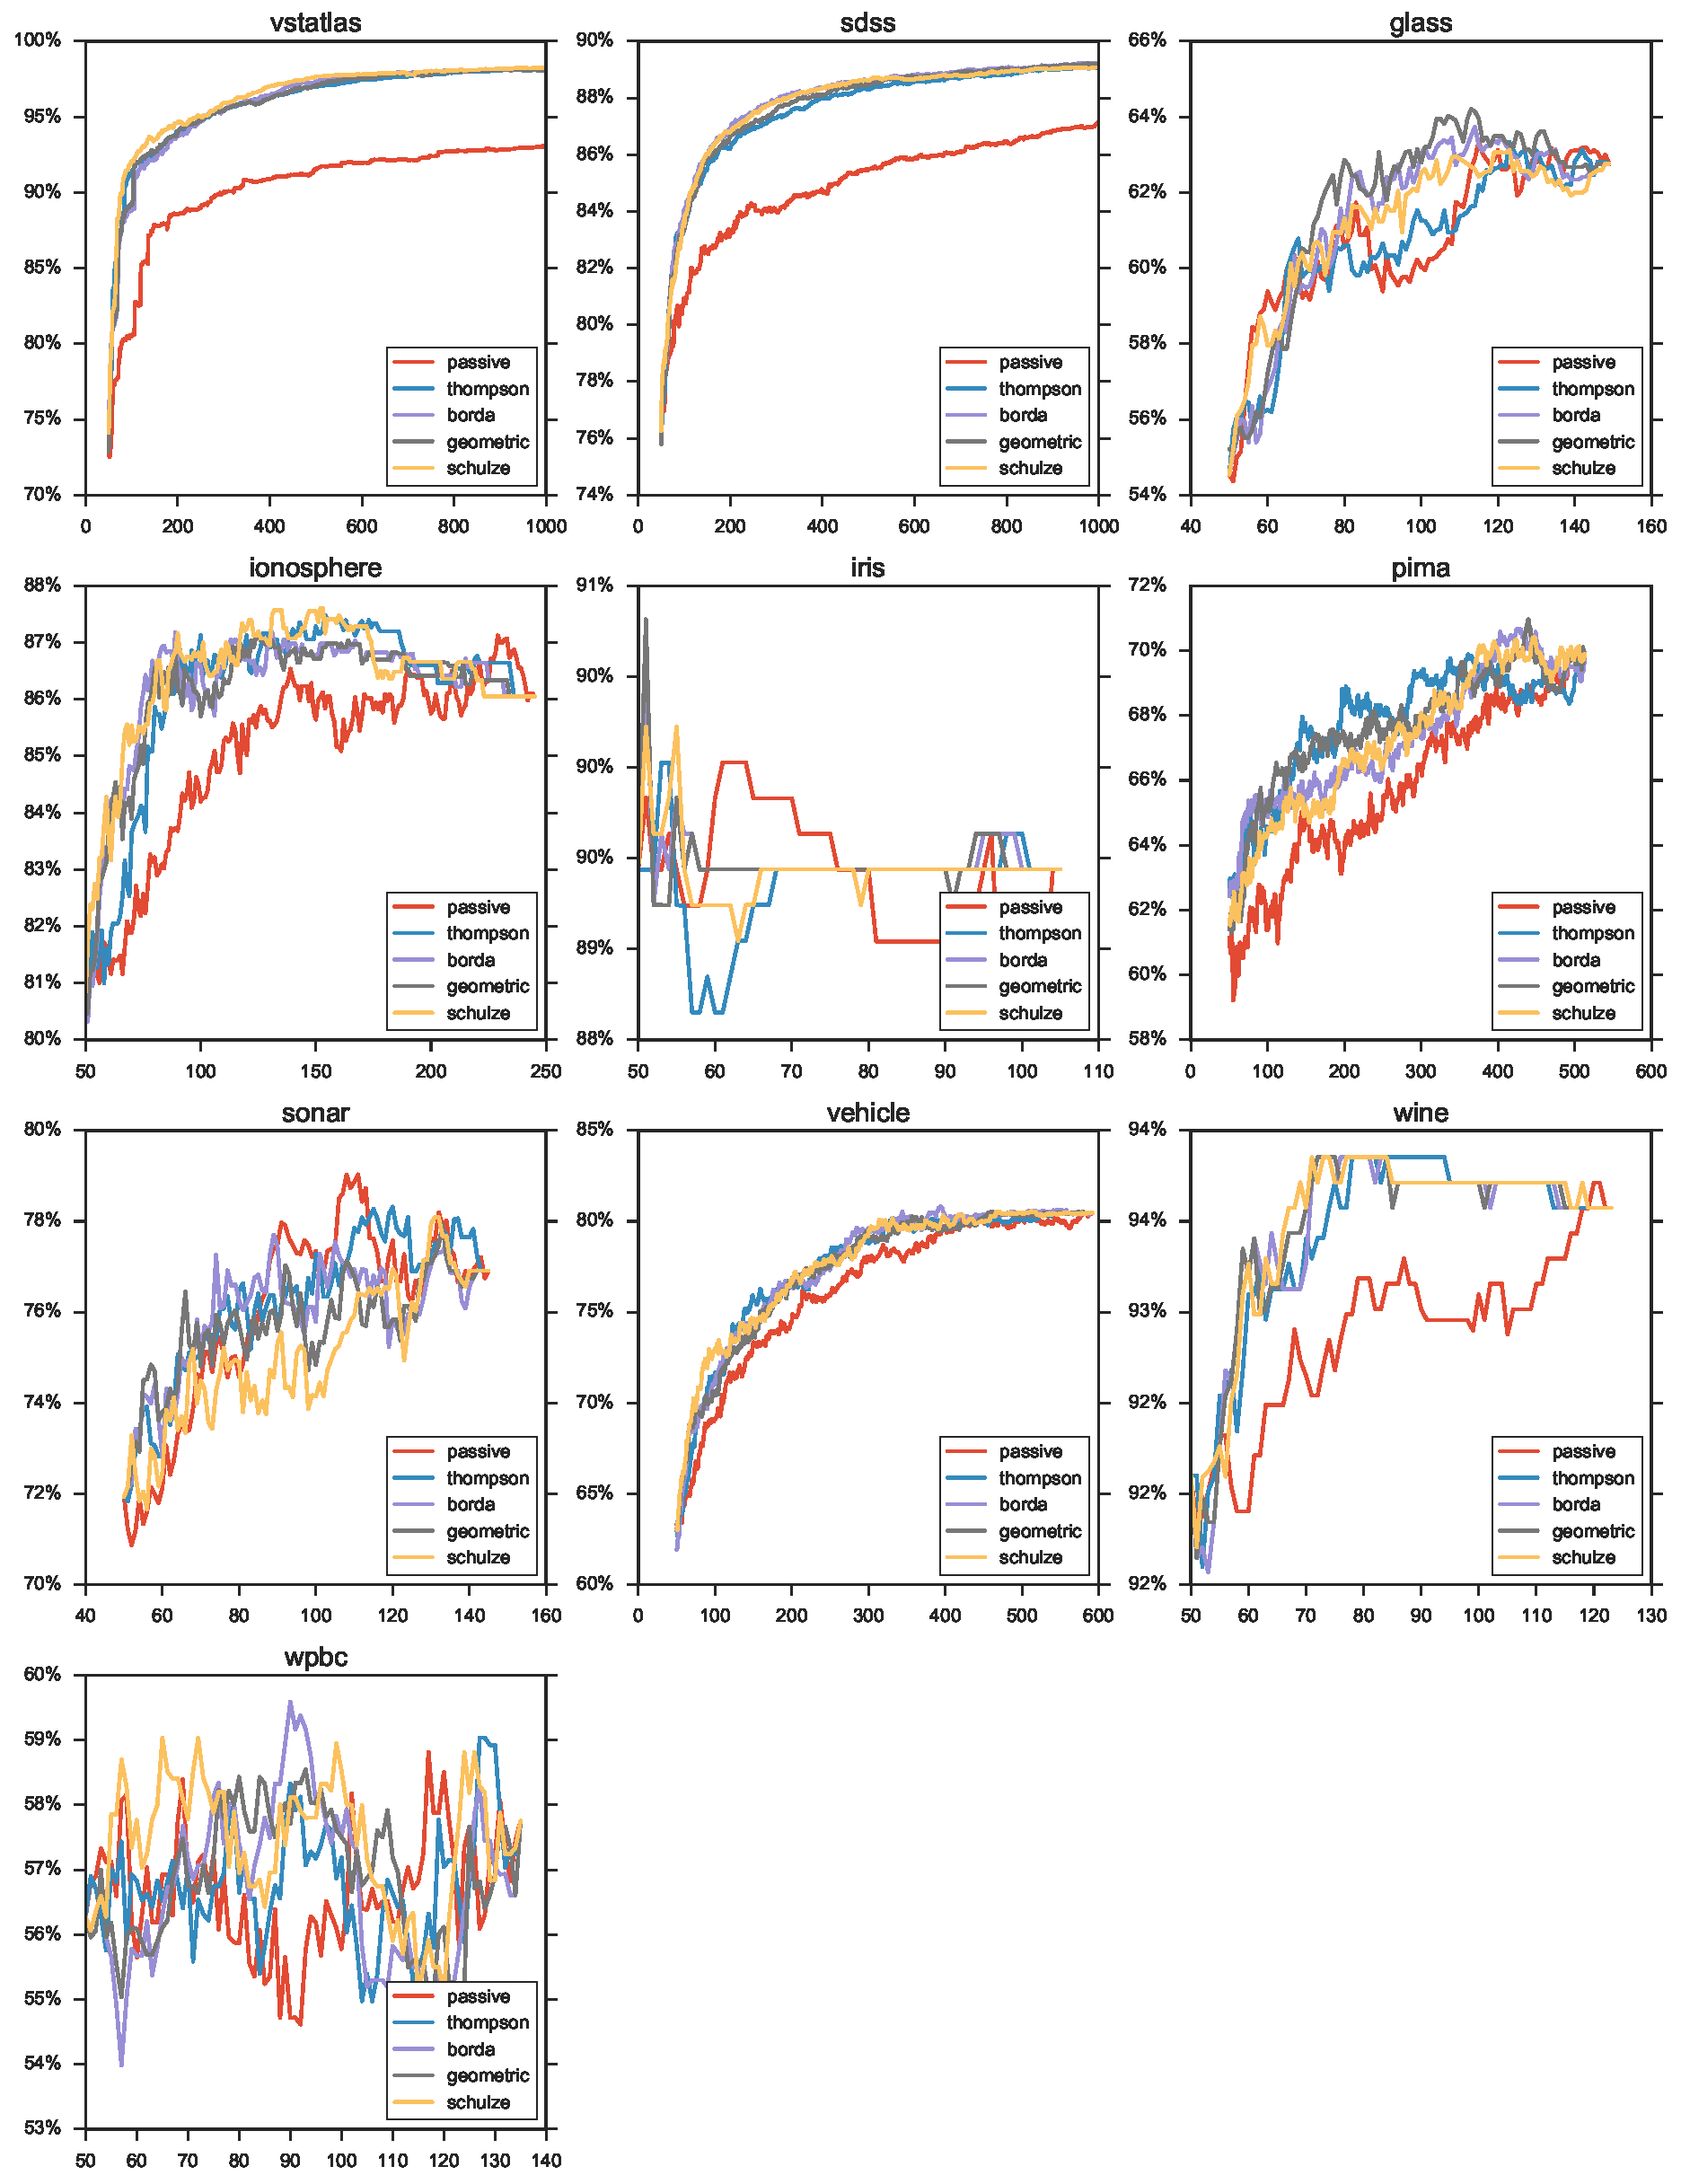
\includegraphics[width=\textwidth]{figures/learning_curves}
	\caption[Selected learning curves]{Selected learning curves.}
	\label{fig:learning_curves}
\end{figure}


\section*{Acknowledgments}

SDSS

\bibliography{active}

\end{document}
